\documentclass{article}

\usepackage[dutch]{babel}
\usepackage{url,hyperref,enumitem}
\usepackage{aes,cursus,a4wide}
\usepackage{qrcode}

\setlength\parindent{0cm}
\setlength\parskip{1ex}

\setdescription{style=nextline}

\newcommand\meta[1]{\placeholder[#1]}
\newcommand\marg[1]{\cmdarg{\meta{#1}}}

\newcommand\classnaam{aesbrief}
\newcommand\classsf{\textsf{\classnaam}}

\title{Het Donabrief package} %\\{\large versie \fileversion}}
\author{\aeskwadraat \TeXniCie\\
\url{hektex@a-eskwadraat.nl}}
%\date{\filedate}

\begin{document}

\maketitle

\section{Inleiding}
Dit package haalt alle uitgebreide en lastige \LaTeX code weg uit de donabrief en reduceert tot enkele simpele commando's die hier uitgelegd worden. De aanhef en groet staan vast. Deze zijn altijd ``Beste..., '' en ``Met vriendelijke groet, ''.

Net zoals in de normale aesbrief class zul je nog wel de datum en signature goed moeten zetten voordat je \cmd{begin}\cmdarg{document} doet. Dit doe je met de commando's:\cmd{datum}\cmdarg{30 februari 2012} en \cmd{signature}\cmdarg{Lodewijk Cornelisz,\textbackslash\textbackslash Ere CFFR Lid}.

\section{Commands}
\subsection{Inhoud maken}
Om de inhoud van alle delen van je brief te geven kun je de volgende argumenten gebruiken. Gebruik de verschillende delen ook echt all\'e\'en daar waarvoor ze bedoeld zijn, want ze zetten ook gelijk het onderwerp van je brief goed!

\cmd{inleiding}\cmdarg{stukje voor boven aan de brief}

\cmd{afsluiting}\cmdarg{stukje voor boven de met vriendelijke groet}

\cmd{vakidioot}\cmdarg{stukje over de vakidioot}

\cmd{reis}\cmdarg{stukje over het reisverslag}

\cmd{almanak}\cmdarg{stukje over de almanak}

\cmd{jvs}\cmdarg{stukje over het jaarverslag}

\cmd{bonusding}\cmdarg{Bonus stukje} voor alles wat niet onder de bovengenoemde kopjes valt.

\subsection{Inhoud plaatsen}
Geef, nadat je de inhoud gemaakt hebt met de bovenstaande commando's, het \cmd{formateer} commando om de inhoud in de goede volgorde te plaatsen.
\cmd{formateer}\cmdarg{plaatsingscommando's} De inleiding en afsluiting worden al automatisch geplaatst. De commando's om het spul op de goede plek te krijgen zijn als volgt:

\cmd{vakidhier}

\cmd{reishier}

\cmd{almahier}

\cmd{jvshier}

\cmd{jvshier}

\cmd{bonushier}

Zoals de verwachten komen deze commando's overeen met de eerder aangemaakte inhoud.
\section{Voorbeeld}
\begin{figure}
\fbox{%
\begin{minipage}{\textwidth}
\verbatiminput{donabrief-voorbeeld.tex}
\end{minipage}%
}
\caption{Een voorbeeld van het gebruik van donabrief.}
\label{fig:code}
\end{figure}

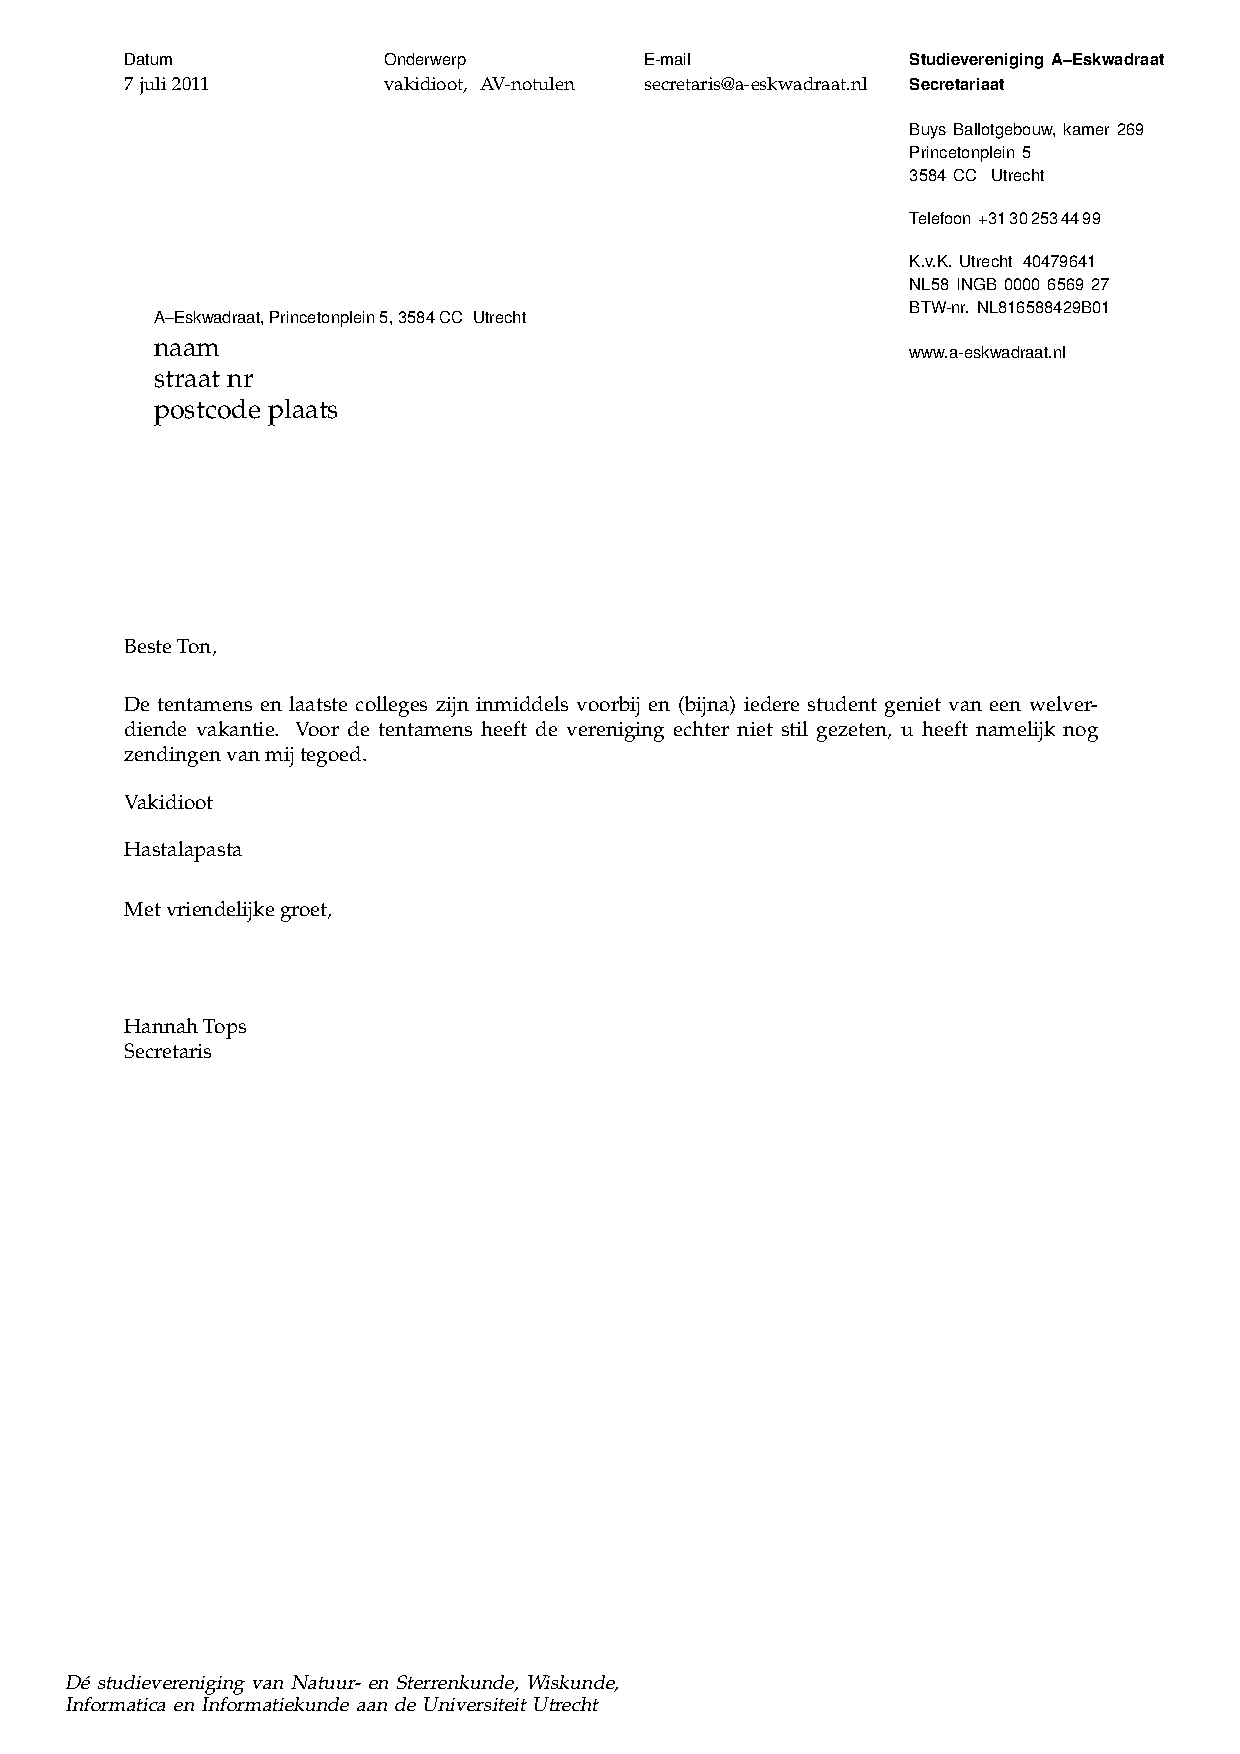
\includegraphics[height=.75\textheight]{donabrief-voorbeeld.pdf}

\end{document}